\chapter{General Semistructured Model and Nested Graphs}\label{cha:graphsdef}
\epigraph{``\textit{The empirical basis of objective science has nothing 'absolute' about it. Science does not rest upon solid bedrock. The bold structure of its theories rises, as it were, above a swamp. It is like a building erected on piles. The piles are driven down from above into the swamp, but not down to any natural or 'given' base; and if we stop driving the piles deeper, it is not because we have reached firm ground. We simply stop when we are satisfied that the piles are firm enough to carry the structure, at least for the time being.}''}{--- Karl R. Popper, \textit{The Logic of Scientific Discovery}, V. 30}

%The previous chapter showed that better performances for graph algorithms can be performed by using an adjacency list representation. This implementation provided better performances that the ones achievable on both relational and graph data storages, and that our proposed query plan performed better solutions that the one provided by current graph query languages. Nevertheless, in 

Chapter \vref{cha:datadef}  addressed the problem of providing nested concepts in current data models. Graph models also proved not to meet such representation goals adequately and, therefore, a new data model for graph nested data is required. On the other hand, semistructured data representations do not allow to represent the containment of one single object by multiple containers, as needed for a possible generalization of the EPGM\index{graph!EPGM} model. Consequently, we choose to   define   a \textsc{Generalized Semistructured data Model}  (\textbf{GSM}\index{GSM|see {General Semistructured Model}}\index{General Semistructured Model}, Section \ref{def:mofgeneral}) on top of which the new nested graph model is going to be subsequently defined (\textbf{nested graphs}\index{graph!nested graphs}, Section \ref{def:ngraph}). 

The present chapter provides some translation functions $\tau$ from the previous data models towards the GSM data model, thus meeting two distinct goals: \begin{mylist}
	\item we show the generality of GSM, that
	\item can be the used within the LAV/GAV \index{data integration!global as a view} \index{data integration!local as a view} data integration scenarios for syntactically $\ttransl$-translating one data model towards the GSM or Nested Graph model.
\end{mylist}
The choice of representing both vertices and edges with ``objects''\index{object} may surprise the reader, because Chapter \ref{cha:datadef} warned against the problem of semantic overloading. The reader must be aware that the implications of the previous paragraph fall only at the representation level of the single element while, on the other hand, the data model should distinguish those different concepts.


\begin{figure}
	\centering
	\begin{minipage}{.45\textwidth}
		\centering
		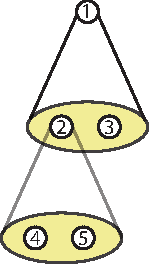
\includegraphics{fig/04model/01SimpleNesting}
		\subcaption{This picture provides a representation of a data structure containing two different nesting levels. Each object is represented by a circle, while
			the containment $\varphi$ function of each object is represented by the cone departing from each object. Within this graphical representation, the leftmost nested object is the first object appearing in the containment function $\varphi$.}
		\label{fig:01simplenesting}
	\end{minipage}\quad \begin{minipage}{.45\textwidth}
		\centering
		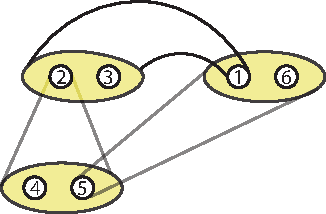
\includegraphics{fig/04model/02RecursiveNesting}
		\subcaption{The data model that is now provided is as general as possible, and hence can support any possible representation. This also implies that recursive nestings are allowed. In particular, this Figure shows that node $2$ may contain elements $4$ and $5$, which contains $6$ and $1$ which contains $2$. Therefore, $\varphi(2)=[4,5]$, $\varphi^2(2)=[1,6]=\varphi(5)$, and $\varphi^3(2)=[2,3]$. This recursive nesting solutions should be avoided for representing aggregations.}
		\label{fig:02recursivenesting}
	\end{minipage}%
	\bigskip 
	
	\begin{minipage}{.45\textwidth}
		\centering
		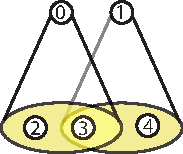
\includegraphics{fig/04model/03Overlapping}
		\subcaption{This picture shows how the $GSM$ model allows to nest one element (e.g. $3$) in more than one single element. In particular, $\phi(0)\cap\phi(1)=[3]$.}
		\label{fig:03overlapping}
	\end{minipage}
	\caption{Different possible instances of the $GSM$ model, allowing arbitrary nestings within its objects. These pictures show some situations that cannot be natively expressed by the current nested relational model and other semistructured representations. In particular, each cone represents one single association between the containing object and its content through an expression $p$.}
\end{figure}
Last, we provide some use cases for both aggregating (Section \ref{subsec:nested-partof}) and integrating (Section \ref{sec:ngusecases}) data representations within the proposed data format. Concerning the last use case, we must   observe that in the third chapter  we  showed that the alignment of types -- which may nest other concepts -- relies on both the successive alignment of other attributes (or nested types) and on the attributes contained inside such types. Given that both types and attributes are involved in the alignment process, it follows that they all must be represented -- within the alignment process -- as objects with a given type represented through labels. 
After this alignment process, edges must be aligned too: this process is required for a complete data integration scenario. Consequently, this chapter introduces the concept of edge alignment for data integration (as previously introduced in Section \vref{sss:ngdi}), thus allowing to provide a first definition of the $\qtransl$ operator as well as $\stigma$  refining the previously mined alignments. Moreover, the same example shows that GSM allows a uniform representation between data models, schemas and alignments.
